\section{Results}
\label{sec:4.2_results}

% 4.2.1
% -----
\subsection{Network overview}
\label{sec:4results_overview}

To train a CNN to predict fluorescence intensity from EM images, we first create training datasets comprised of high-magnification EM and FM image pairs. The FM images are acquired by a fluorescence microscope integrated into the chamber of a scanning electron microscope (SEM) \cite{liv2013simultaneous, zonnevylle2013integration}. This instrumental setup allows for [sub-\SI{10}{\nano\meter} overlay precision without a reliance on fiducial markers or manual input \cite{haring2017automated}.] The lack of fiducial markers is beneficial as the network does not learn on extrinsic markers, while the lack of manual input enables the accumulation of correlative datasets to be partially automated and scalable to several GBs. A more detailed description of how integrated CLEM datasets are generated can be found in \ref{sec:2methods_acqstrat} as well as in \textcite{lane2021optimization}.

GB-sized image data is far too cumbersome for modern deep learning models to train on. The registered image data is therefore divided into small tiles which serve as input for the model (Figure \ref{fig:4.1_overview}A); the model architecture can be adjusted to support an arbitrary number of fluorescence channels. The image tiles are shuffled around to diversify the [area thereby avoiding overfitting]. A multi-layer CNN was chosen to train on due to its proven ability for recognizing structural detail in EM image data [and its performance in superhuman pattern recognition] (Figure \ref{fig:4.1_overview}B). To address the resolution mismatch between EM-FM image pairs, the model is designed with more contraction paths than expansion paths---resulting in an elongated, backwards ``J"-shape, as opposed to the more characteristic ``U". Once trained, the model is able to generate predictions of the fluorescence intensity on individual EM image tiles. Separate correlative EM-FM datasets are set aside for validating and testing the model. By stitching together the [model's output] it is possible to [render] large-scale or volume predictions of the fluorescence intensity. These can be superimposed onto the EM test dataset to generate large-scale or volume CLEM predictions (Figure \ref{fig:4.1_overview}).

% We train and test network to [list all the samples...]


% Figure 4.1 (overview)
% ---------------------
\begin{figure}[!tbh]
    \centering
    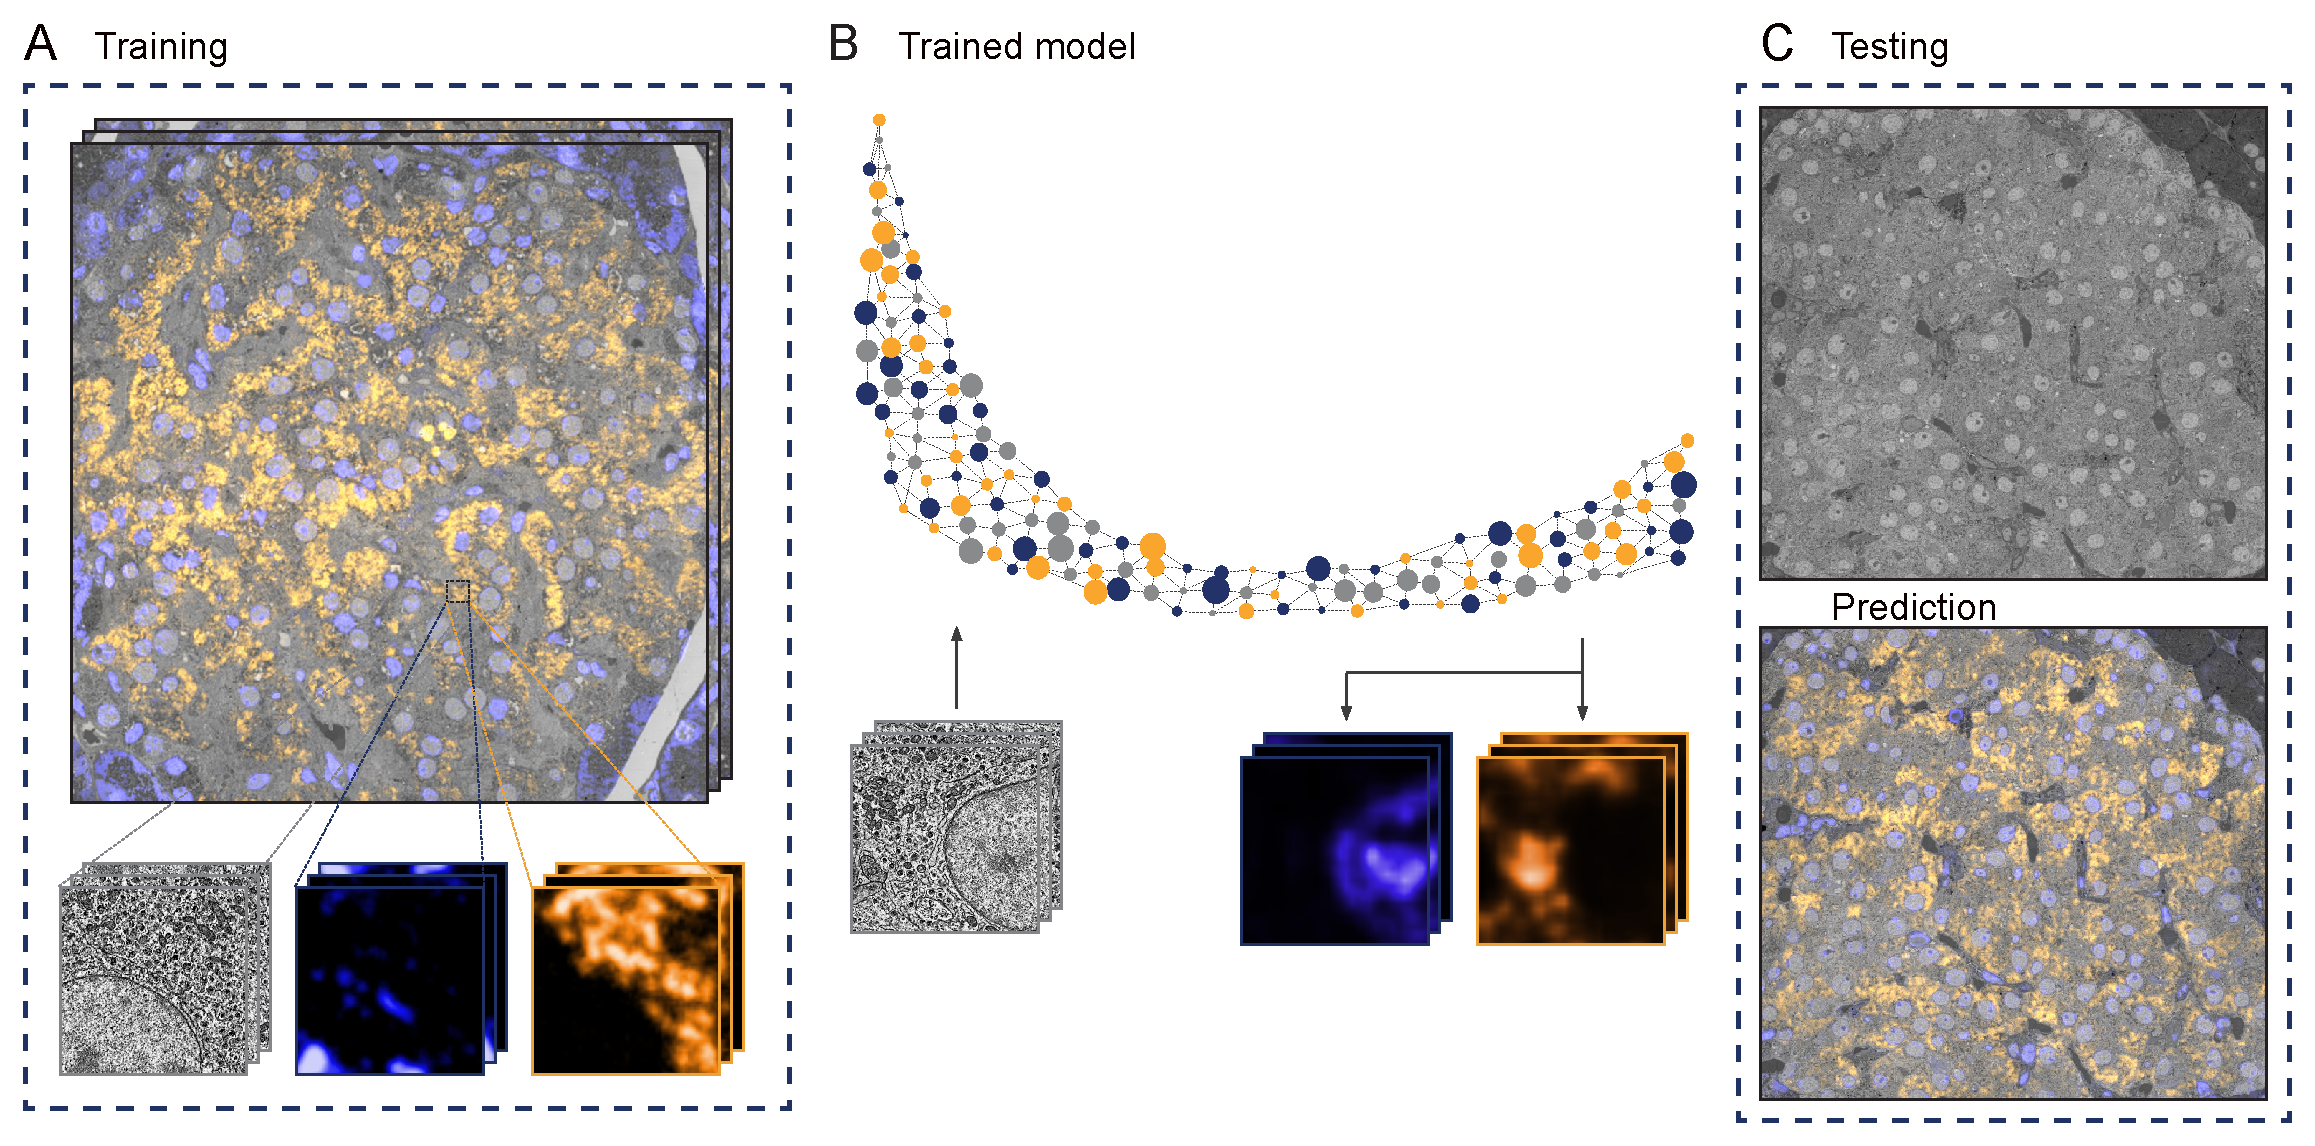
\includegraphics[width=\linewidth]{chapter-4/figures/fig1_overview_v5.pdf}
    \caption{\textbf{Overview of procedure for fluorescence intensity predictions.}
    Training data for the model consists of registered, large-scale CLEM datasets (A) comprised of high-magnification EM images and an arbitrary number of fluorescent channels. For the rat pancreas tissue shown here, the fluorescent channels consist of a Hoechst stain, targeting cell nuclei, and an AF594 immunostaining, targeting insulin granules. CLEM image data is input into an asymmetric convolutional neural network (B) which maps the EM image data to FM image data. The model is represented by an elongated, backwards J-shape as it consists of fewer upsampling layers than downsampling layers---a result of the resolution difference between the EM and FM images. Once trained, the network generates predictions from large-scale EM data (C) such that the generated predictions can be overlaid with the input EM data to generate large-scale correlative datasets of the predicted fluorescence (D).
    \textbf{[TODO: add scale bars.]}}
    \label{fig:4.1_overview}
\end{figure}



% 4.2.2
% -----
\clearpage
\subsection{Network predictions on thin tissue sections}
\label{sec:4results_pancreas}

To characterize the performance of our network, we first apply it to sections of rat pancreas tissue. The tissue is given a Hoechst stain---targeting cell nuclei---as well as immunolabelled with AF594---targeting insulin granules. The predicted fluorescence signal (green) is found to correlate well with the true fluorescence (red) (Figure \ref{fig:4.2_pancreas}). When applied to an entire islet of Langerhans, the network registers Pearson correlation coefficients (PCC) of 0.67 and 0.76 for the predicted Hoechst and AF594 signals respectively. At high magnification, the predicted signals are found to exhibit a close qualitative resemblance (Figure \ref{fig:4.2_pancreas} insets). Notably, the true Hoechst fluorescence is more heavily concentrated along the nuclear envelope, whereas the predicted Hoechst signal is relatively stronger in regions of denser chromatin. The predicted AF594 signal matches well with that of the true fluorescence with the caveat that it appears somewhat blurred, likely due to the insulin granules themselves being diffraction-limited. There are other factors that may contribute to a diminished PCC that are extraneous to the network. These include bleedthrough of one fluorescence channel into another (Supplemental Figure \ref{fig:4.S1_rois}B), errors in the EM-FM registration (Supplemental Figure \ref{fig:4.S1_rois}C), and aberrations in the true fluorescence microscopy images (Supplemental Figure \ref{fig:4.S1_rois}D). Not only do these examples help justify a reduced correlation coefficient, but they demonstrate the network's ability to effectively correct for imperfections in the true fluorescence signal.


% Figure 4.2 (pancreas)
% ---------------------
\begin{figure}[!tbh]
    \centering
    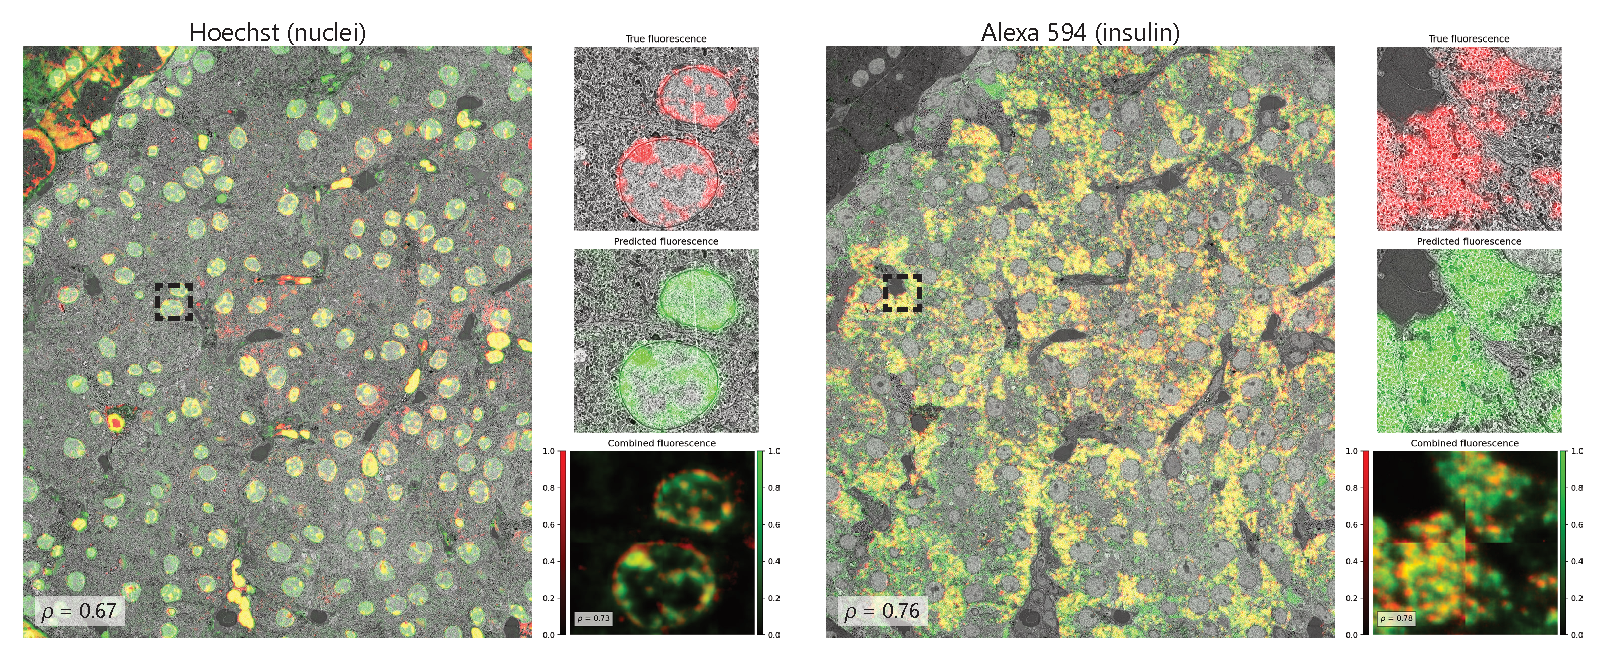
\includegraphics[width=\linewidth]{chapter-4/figures/fig2_pancreas_v11.pdf}
    \caption{\textbf{Network predictions of Hoechst and AF594 fluorescence intensity show high fidelity with respect to the true fluorescence signal.}
    Network predictions are applied to sections of rat pancreas tissue (left). The predicted fluorescence signal (green) correlates well with---and in many instances---overshadows the true fluorescence signal (red).
    Insets show typical network prediction results at full resolution.
    The prediction for the Hoechst signal shows high confidence in expected intensity in regions where the chromatin (revealed by EM) is most dense, correlating well with the true fluorescence signal ($\rho=0.74$).
    The network prediction for AF594 is likewise highly correlated to clusters of insulin granules ($\rho=0.79$).
    \textbf{[TODO: Bigger PCC box. Possibly enlarge insets. Add scale bars.]}}
    \label{fig:4.2_pancreas}
\end{figure}



To further characterize the performance of the model, we assess human recognition of cell nuclei in the network-generated fluorescence signal versus the true fluorescence (Figure \ref{fig:4.3_counting}). In order to quantify recognition in fluorescence, a ground truth set of cell nuclei based on EM data from the same region is first established (Figure \ref{fig:4.3_counting}A). Approximately 200 cell nuclei were manually annotated by a combination of experts and trained volunteers. Unsupervised brute-force nearest neighbors was used to filter out spurious annotations. $k$-means clustering was then used to partition the remaining annotations into clusters of point clouds. The centroids of these point clouds were computed and used to localize the nuclei from which the ground truth set was determined (see Section \ref{sec:4methods_analysis} for details).
Experts and trained volunteers were then asked to recognize cell nuclei in the true and predicted fluorescence datasets (Figure \ref{fig:4.3_counting}B). Nuclei are considered to be correctly identified (true positive, TP) when they are detected within a certain threshold distance from a nucleus in the ground truth set. This threshold is approximately the average cell nucleus diameter. Incorrectly identified nuclei---points for which there is no nearby nucleus---are considered to be false positives (FPs), while those that are missed entirely are considered to be false negatives (FNs).
The precision, recall, and F1 score are calculated for each individual [annotation] and then averaged (Figure \ref{fig:4.3_counting}C). Similar precision scores for the true (72\%) and predicted (74\%) fluorescence datasets suggest that a comparable number of false positives were identified in both, while the notably higher recall for the predicted dataset (80\% vs 58\%) indicates that a substantially higher number of cell nuclei become recognizable from the predicted signal. This can be seen throughout the dataset (Figure \ref{fig:4.3_counting} inset), but is particularly noticeable in the outer regions where the true fluorescence signal is somewhat weaker due to imperfect illumination and the nuclei become somewhat obscured due to Hoechst expression from RNA in the endosplasmic reticulum.
The notably higher F1 score for the predicted dataset (76\%\ vs 64\%) demonstrates the improved recognition ability afforded by the predicted signal.
The same assessment cannot be done for insulin granules as the typical size is ${\sim}\SI{100}{\nano\metre}$---well below the diffraction limit. Hence individual granules are too difficult to distinguish by eye.

% somehow acknowledge that this is kind of backwards / a weird thing to do -- maybe in the discussion


% Figure 4.3 (counting)
% ---------------------
\begin{figure}[!tbh]
    \centering
    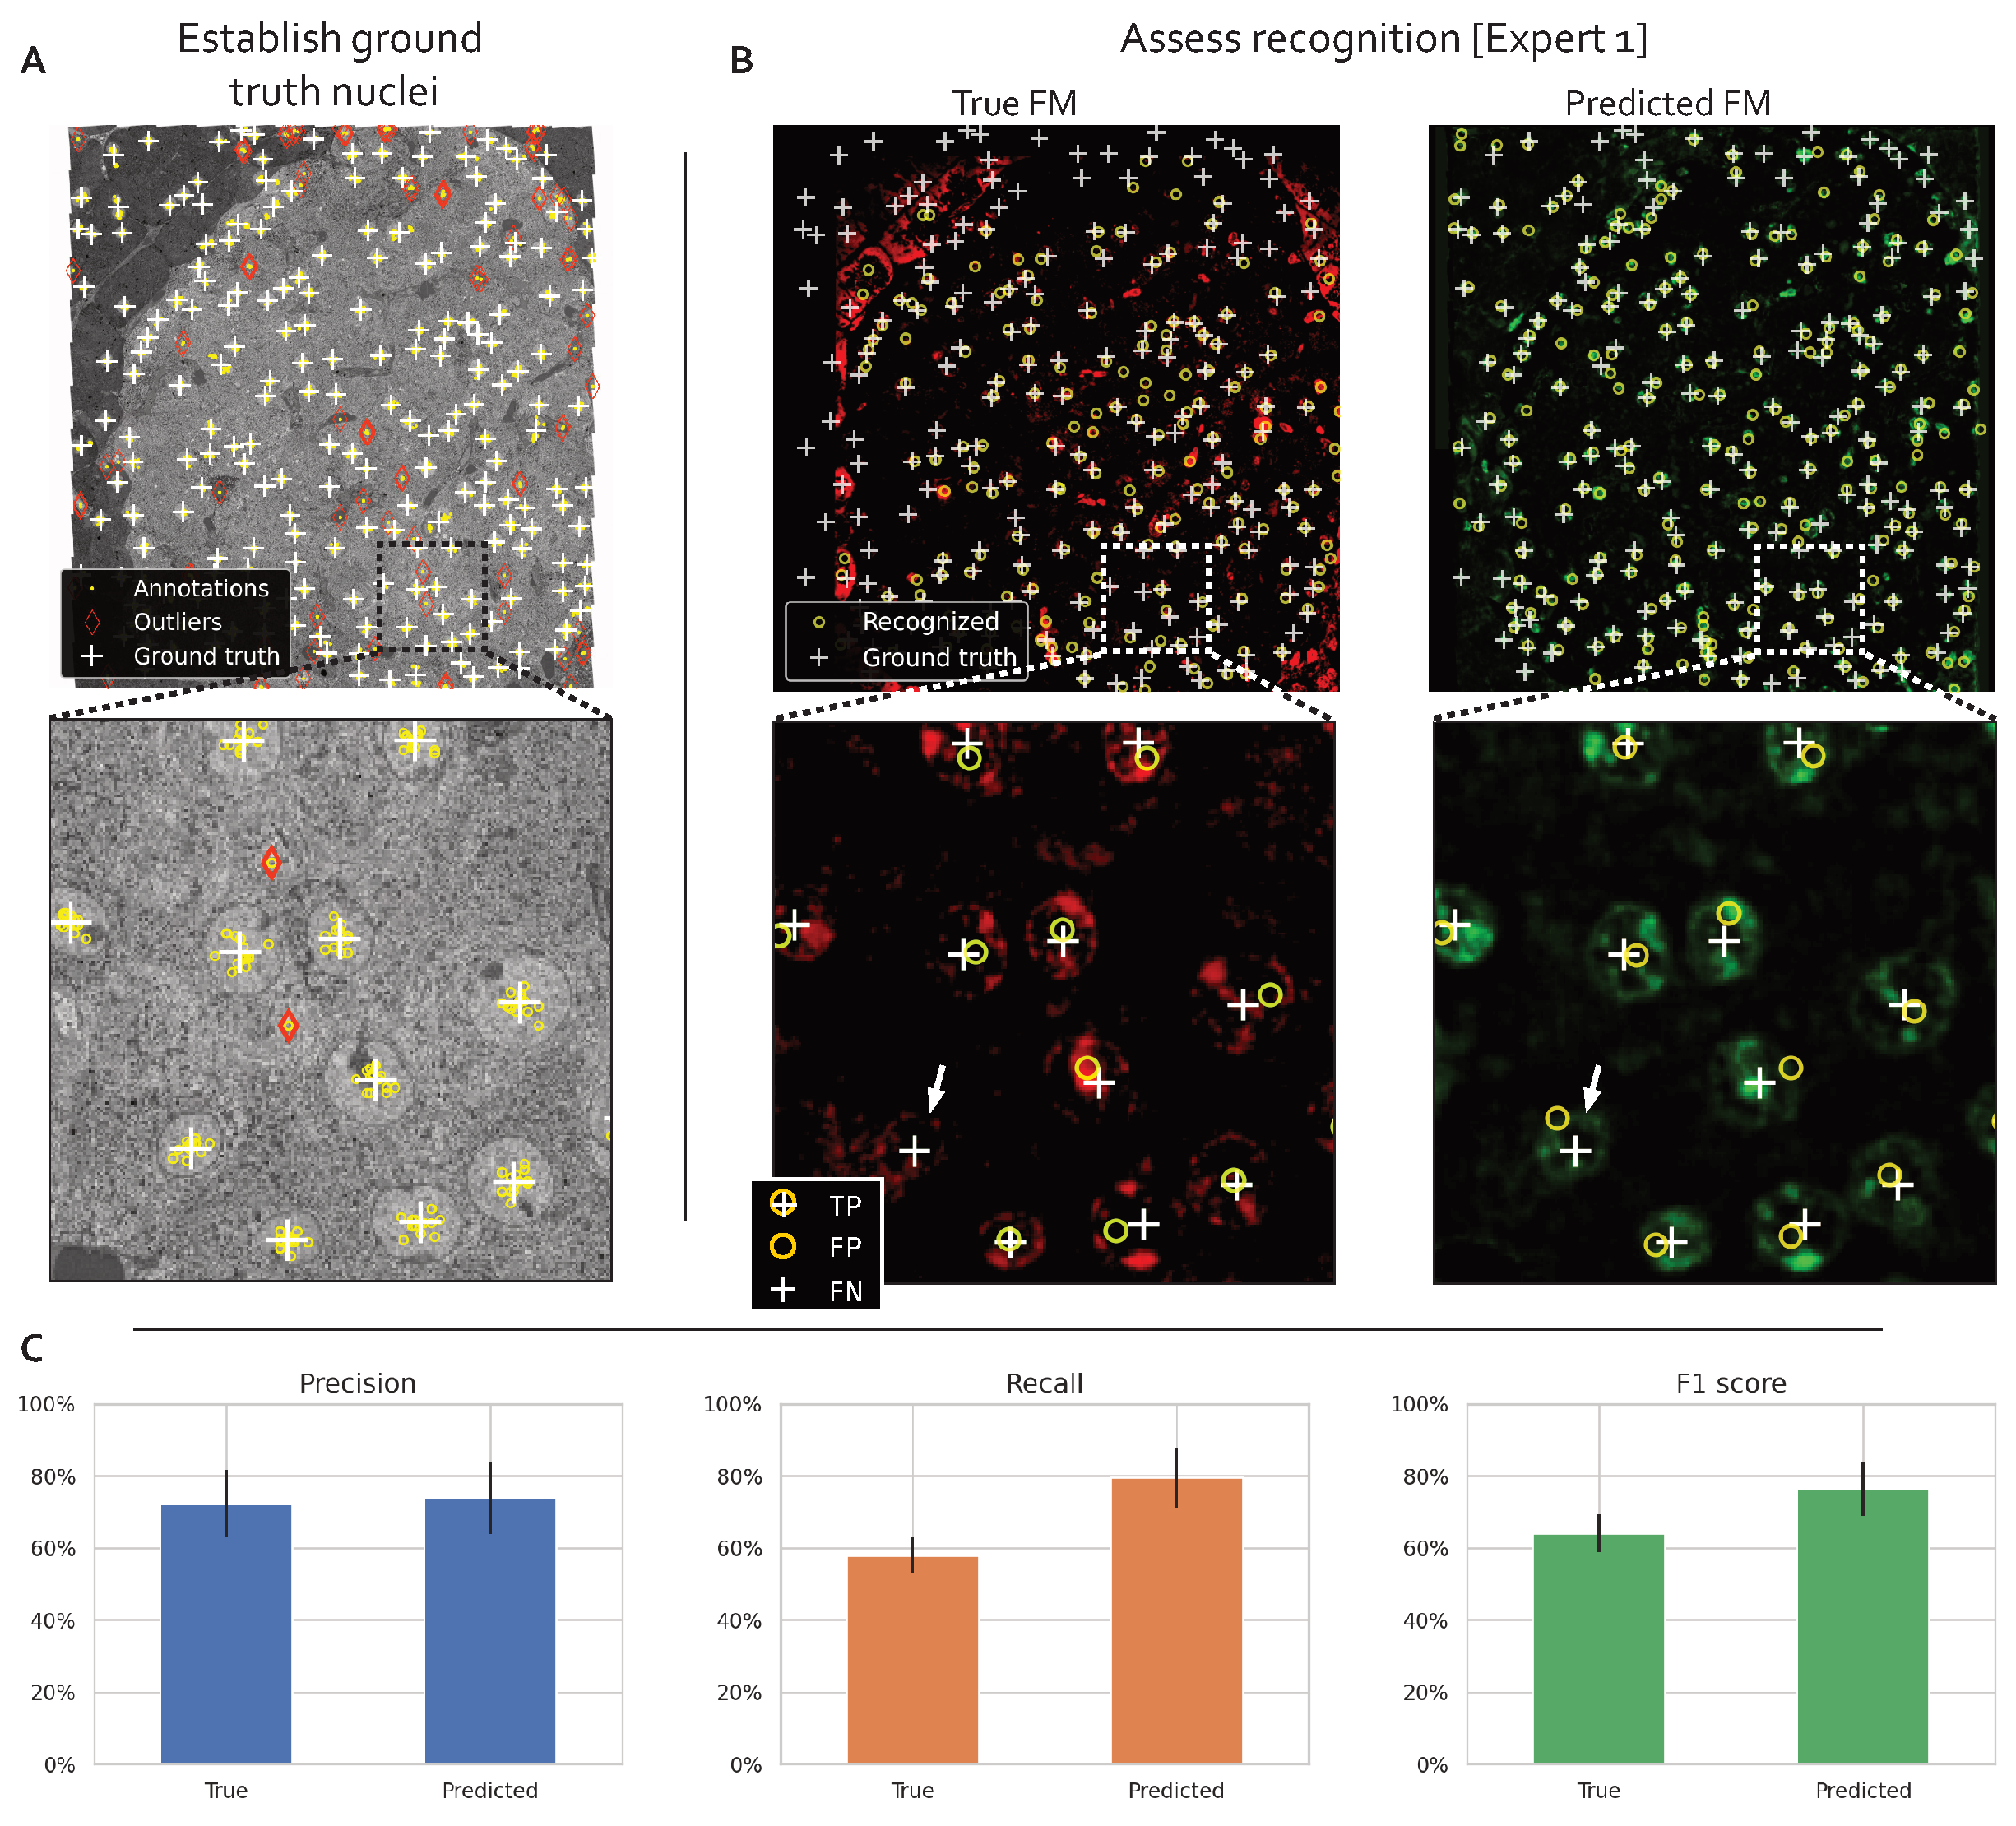
\includegraphics[width=\linewidth]{chapter-4/figures/fig3_counting_v3.pdf}
    \caption{\textbf{Predicted fluorescence signal improves human recognition of cell nuclei.}
    (A) An EM dataset is used to establish a ground truth set of cell nuclei. Annotations from a combination of experts and trained volunteers are aggregated using a combination of brute-force nearest neighbors and $k$-means clustering. The ground truth (white crosses) is comprised of nuclei that have been selected by a majority of annotators, while outliers (red diamonds) were thrown away.
    (B) An individual recognition of cell nuclei in the true and predicted fluorescence datasets is evaluated against the established ground truth. A yellow circle marks where the observer has identified a nucleus. Correctly identified nuclei (true positives, TP) are therefore denoted by an overlapping white cross and yellow circle, while incorrectly marked nuclei (false positives, FP) and missed nuclei (false negatives, FN) are denoted by a solitary yellow circle and solitary white cross, respectively. Arrows indicate an instance of a cell nucleus that went unrecognized in the true fluorescence image (FN), but was identified in the prediction (TP). This can be attributed to the lack of background in the predicted fluorescence signal.
    (C) All of the individual annotations are aggregated to calculate the mean precision, recall, and F1 score.
    \textbf{[TODO:]}}
    \label{fig:4.3_counting}
\end{figure}



% 4.2.3
% -----
\subsection{Network predictions on cells (tentative)}
\label{sec:4results_cells}

\textit{
Possibly (HeLa) cells labelled with mito-mEosEM embedded in R221. Awaiting sample\ldots
}




% 4.2.4
% -----
\subsection{Network robustness}
\label{sec:4results_robustness}

We questioned the network's ability to make fluorescence predictions from EM data acquired with different imaging settings. To address this question, we first acquired CLEM data from serial sections of Hoechst-stained HeLa cells embedded in lowicryl HM20. Ten regions from three different sections were acquired with the same imaging settings to establish a baseline set of imaging parameters for the training data (Table \ref{tab:4.2_params_zf}; non-shaded rows). The training dataset was supplemented with CLEM data from the rat pancreas tissue (Hoechst channel only), which was also acquired with the same baseline settings. Individual imaging parameters were then adjusted for subsequent CLEM acquisitions of additional regions of HeLa cells (Table \ref{tab:4.2_params_zf} shaded rows). Section S006B, for instance, was acquired with an increased landing energy (\SI{3000}{\electronvolt} vs \SI{1500}{\electronvolt} baseline).

Fluorescence intensity predictions were made on \SI{1}{\micro\second} EM data in order to assess the network's ability to generate predictions on lower signal-to-noise ratio (SNR) images (Figure \ref{fig:4.4_robustness}A). The predicted fluorescence shows good qualitative agreement with the true fluorescence, suggesting the model is moderately robust to noise. EM image data was augmented with a varying degree of Poissonian noise during training specifically for this purpose (see Section \ref{sec:4methods_augment}). The predicted intensity is clearly localized to the nuclei in spite of moderate sectioning artefacts, which result in stripes through the EM image. The relatively poor PCC (0.23) is due in large part to autofluorescence of the resin, which is completely anti-correlated with the predicted fluorescence intensity.
% autofluorescence more present in HeLa cell sample where there is more bare resin between cells than in tissue.

Fluorescence predictions on \SI{1}{\kilo\electronvolt} EM data demonstrate high qualitative and quantitative agreement with the true fluorescence (Figure \ref{fig:4.4_robustness}B). There was at least one instance where the network was deceived by a ring-like formation of an [unknown organelle]. While cell nuclei are typically much larger than this [mysterious organelle], many small nuclei exist throughout the training dataset as the thin section is essentially a two-dimensional slice through a random plane in the cells.
The network is also capable of predicting cell nuclei on EM images acquired with larger pixel sizes (Figure \ref{fig:4.4_robustness}C), demonstrating some measure of scale invariance. [It is unknown why the autofluorescence was not consistent throughout the resin]. EM image data is augmented with random affine transforms (see Section \ref{sec:4methods_augment}) to assist in building up this invariance. The relatively poor PCC is again effected negatively by autofluorescence of the resin present in the true fluorescence image.


% Figure 4.4 (robustness)
% -----------------------
\begin{figure}[!htb]
    \centering
    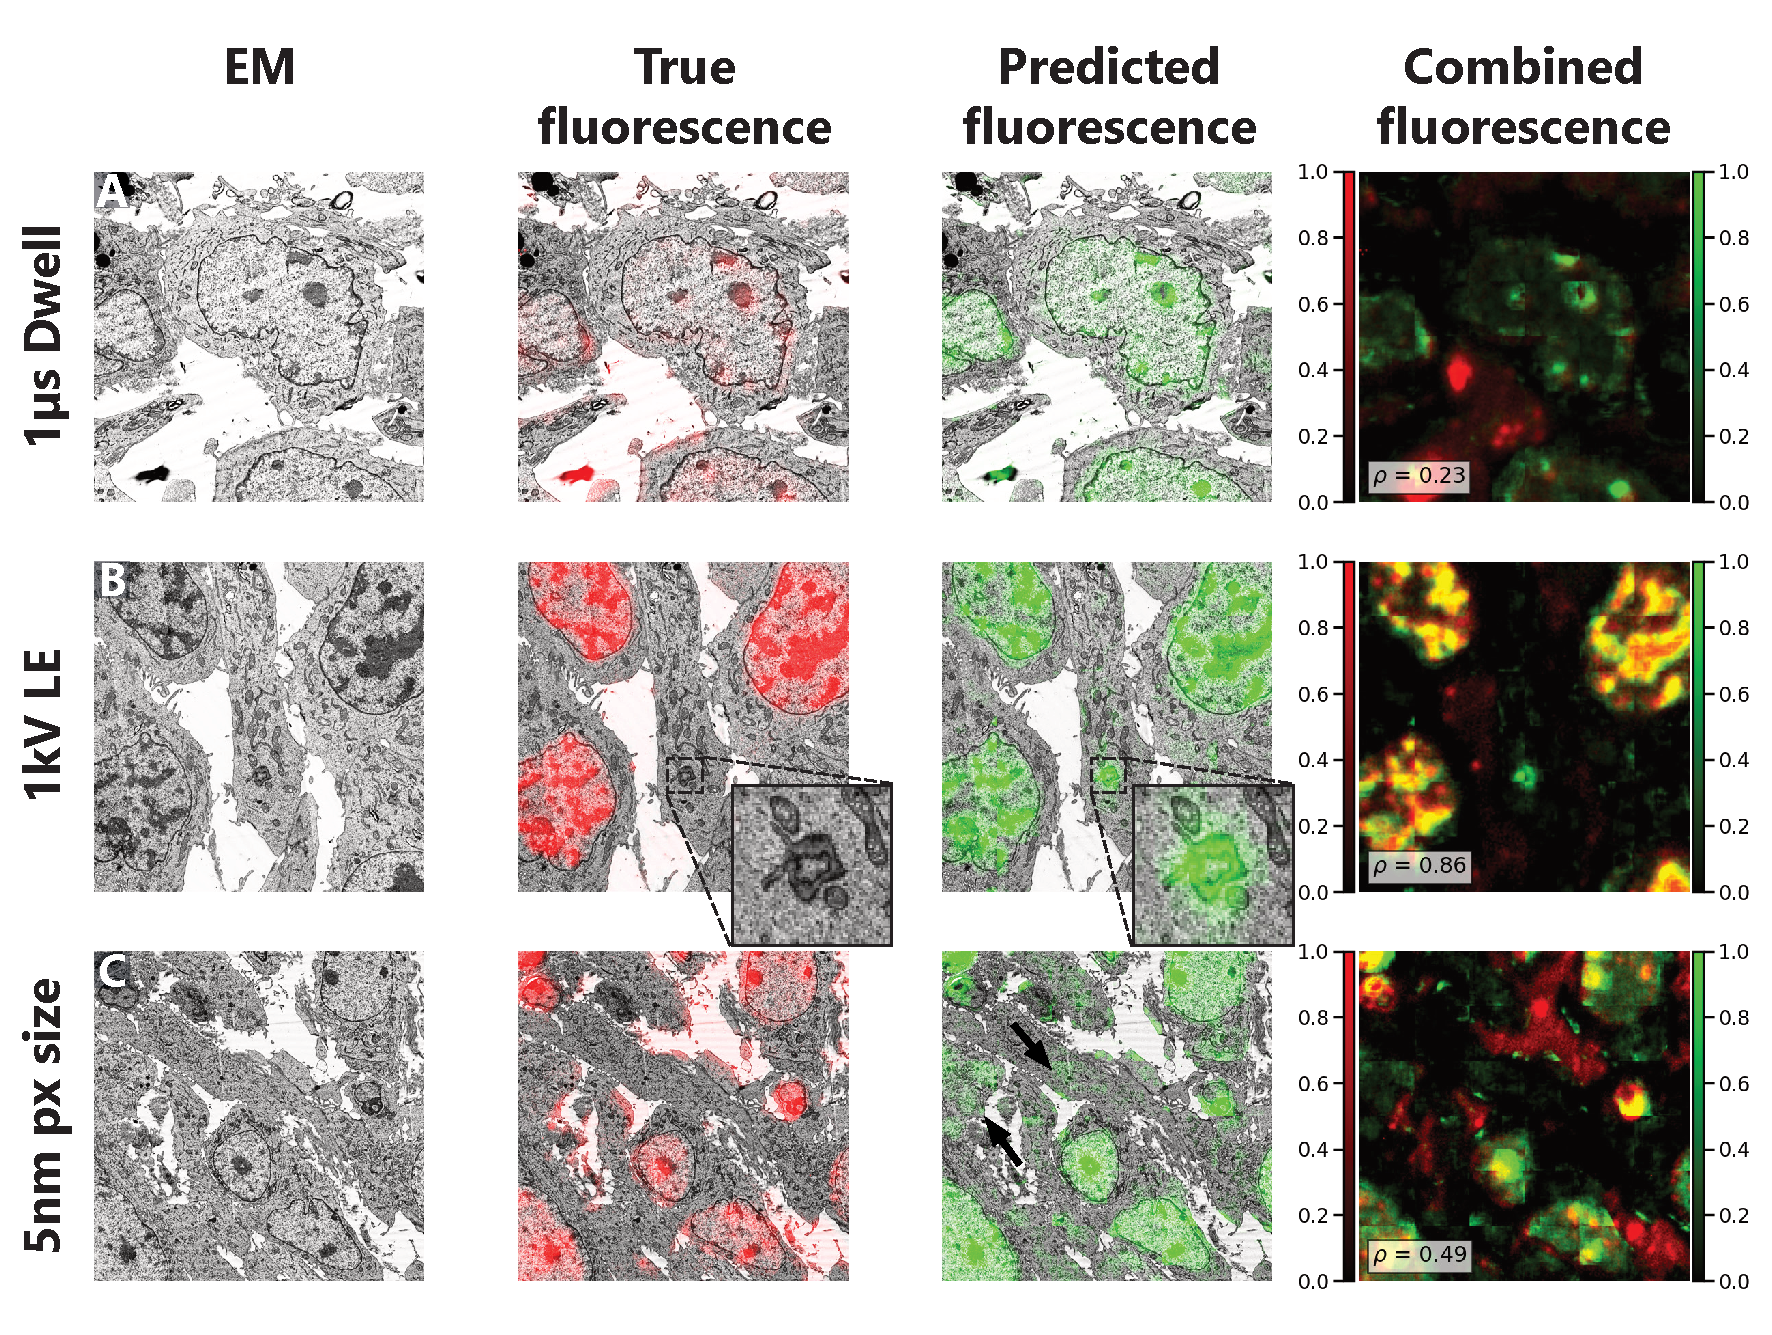
\includegraphics[width=\linewidth]{chapter-4/figures/fig4_robustness_v2.pdf}
    \caption{\textbf{Fluorescence predictions are robust to low SNR EM images as well as those acquired with different imaging settings.}
    Fluorescence predictions were generated on EM images of resin-embedded HeLa cells acquired with a variety of different EM imaging settings.
    (A) Predictions on \SI{1}{\micro\second} EM data are localized to cell nuclei, despite both lower SNR and the presence of sectioning artefacts (striped pattern) in the image. Weak quantitative correlation ($\rho=0.23$) is caused primarily by autofluorescence in the true fluorescence image---seen prominently in the combined fluorescence image.
    (B) Fluorescence predictions on \SI{1}{\kilo\electronvolt} landing energy show high qualitative and quantitative agreement ($\rho=0.86$). Insets show ring-like formation of [unknown organelle] which the network mistakes for an [out-of-plane] cell nucleus.
    (C) Network displays robustness to changes in scale. Fluorescence predictions on EM images acquired with a larger pixel size also exhibit high qualitative agreement. Relatively poor quantitative agreement is again due to autofluorescence of the resin.
    \textbf{[TODO:Add scale bars.]}}
    \label{fig:4.4_robustness}
\end{figure}


% 4.2.5
% -----
\clearpage
\subsection{Weakly supervised, semi-automated segmentation}
\label{sec:4results_segmentation}

We posited that the correlative fluorescence data could facilitate segmentation of targeted organelles. To test this hypothesis, we deployed an instance of ResNet-34 \cite{he2016deep} to perform organelle segmentation. In order to train a neural network to perform organelle segmentation, the model must be provided with labelled images. Typically this is done by manually segmenting hundreds if not thousands of EM images by hand such that the network has a wide variety of examples to learn from. While this method has been shown to be extremely effective, it is also extremely time consuming [references]. To expedite the process for generating labelled image data, we started by simply thresholding the fluorescence images to use as segmentation masks for training (Figure \ref{fig:4.5_masks}). Pixels are classified as either nucleus (cyan) or background (black).

% Figure 4.5 (masks)
% ------------------
\begin{figure}[!tbh]
    \centering
    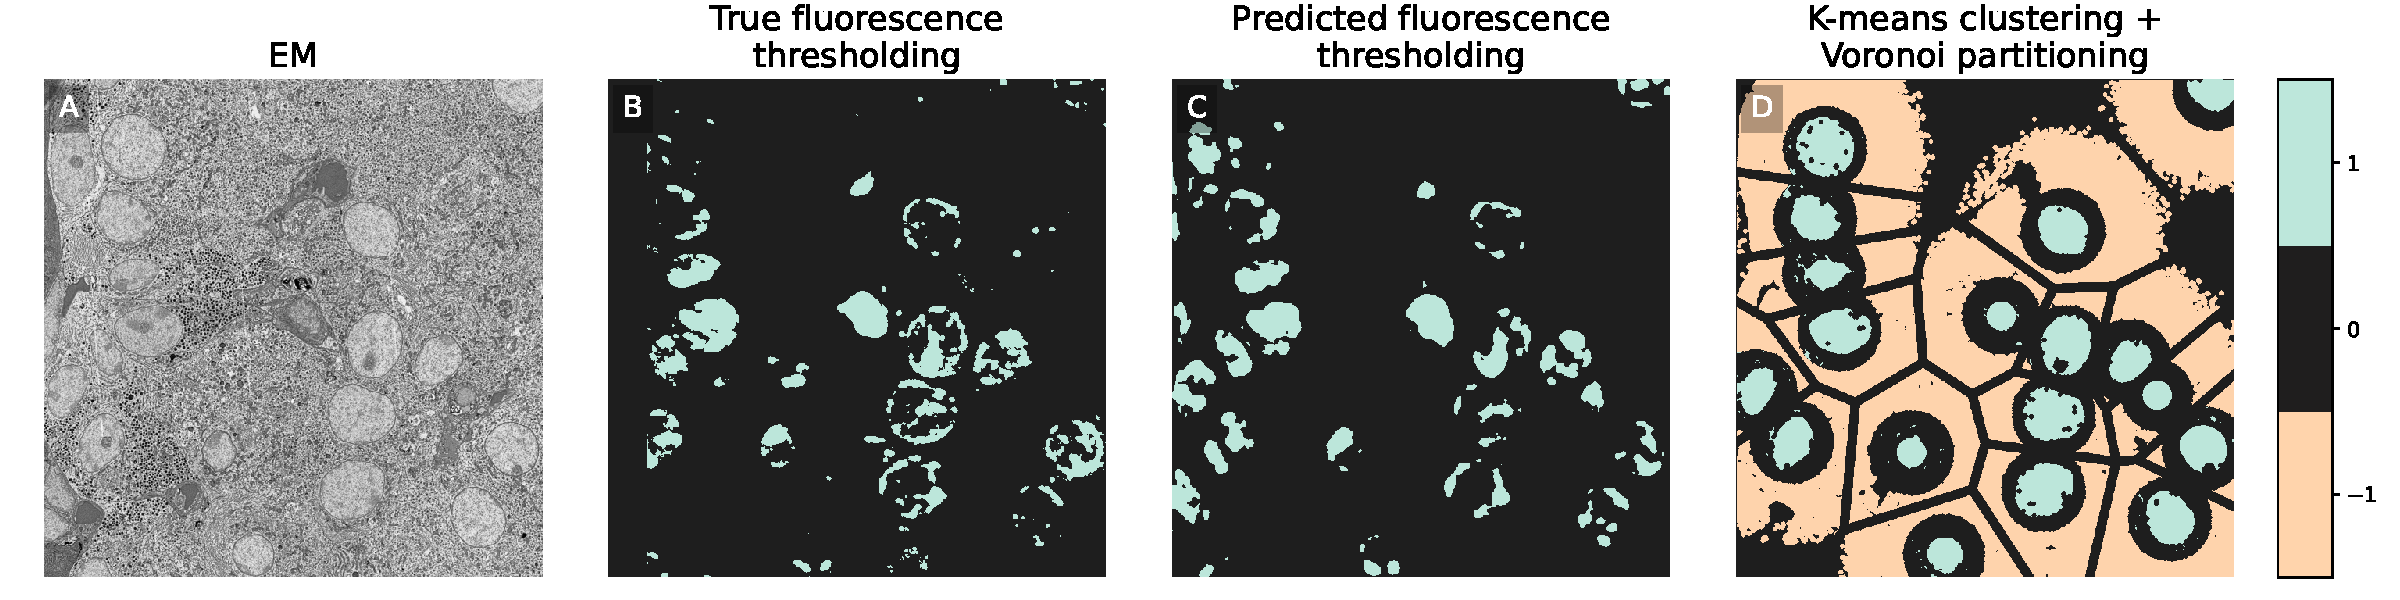
\includegraphics[width=\linewidth]{chapter-4/figures/segmentation_masks.pdf}
    \caption{\textbf{Different labelling strategies employed for CNN-based nuclei segmentation.}
    A) EM image in need of labels for cell nuclei. B) Labelled image derived from thresholding a correlative FM image. C) Labelled image derived from thresholding the predicted fluorescence signal for the corresponding EM image. D) Labelled image derived from a combination of k-means clustering and Voronoi partitioning of the corresponding EM image. The points used in the Voronoi partition are the centroids of nuclei detected by a separate CNN that has been trained based on partial points annotation.
    \textbf{[TODO: Add scale bars.]}}
    \label{fig:4.5_masks}
\end{figure}

It was known that such an approach would result in a significant amount of incorrect labels due to many of the issues mentioned previously---aspecific labelling, FM-EM registration errors, autofluorescence, etc. Because the incorrect labels would be uncorrelated, however, we suspected that ResNet-34 could overlook them in the same way as for the fluorescence predictions (Supplemental Figure \ref{fig:4.S1_rois}). The more profound problem with this simple approach is that the fluorescence signal is typically not uniformly distributed throughout an organelle. In cell nuclei, for example, the fluorescence from the Hoechst staining is localized to the nuclear envelope and chromatin-dense subregions. The result from training ResNet-34 on these masks is hence a fragmented segmentation that largely resembles the fluorescence prediction itself (Figure \ref{fig:4.6_segmentation}C). This is in contrast to segmentation results from the traditional approach---training the network on manually segmented nuclei (Figure \ref{fig:4.6_segmentation}B).

As [CLEMnet] was found to predict fluorescence more uniformly throughout the nucleus, we also experimented with generating labelled images by thresholding the predicted fluorescence data. However, the segmentation results were comparable to those that derived from thesholding the true fluorescence data (Figure \ref{fig:4.6_segmentation}D). While some nuclei are flood-filled, reflecting a successful segmentation, these occurrences are highly inconsistent. The intersection over union (IoU) results underscore the vast difference in segmentation performance. Typical IoU scores for ResNet-34 trained on manually segmented nuclei typically exceed \SI{90}{\!\percent}, while those for ResNet-34 trained on thresholding the true and predicted fluorescence signal are in the range \SIrange{30}{60}{\!\percent}. Hence, a more sophisticated approach for generating labelled images is required.

To generate higher fidelity labelled images, we adapted the method from \textcite{qu2020weakly}. Their method employs partial points annotation to segment cell nuclei from histology images in a weakly supervised fashion. Partial points annotation was deemed appropriate for our purposes as it involves simple selection of target organelles, which is facilitated by a fluorescence overlay. Compared to conventional hand-tracing of organelles, partial point annotation requires only a single point to be selected from a sample of organelles within each image. Thus, it constitutes the annotation method requiring the least amount of manual time and effort, while still providing human-assisted supervision.

Labelled images are generated in a two-phase process. In the first phase, pixels are classified as either nucleus, background, or remain unlabelled, based on the partial points annotation. Mask images of annotated nuclei are created from this classification scheme from which a CNN is trained to detect individual nuclei.
In phase two, labelled images are generated by a combination of k-means clustering and a Voronoi partitioning of the image by the nuclei detected in phase one (see Section \ref{sec:4methods_segmentation} for details). These two types of labels are complementary to one another. K-means clustering preserves the spatial information in the EM image, providing the contour of the nuclei at the expense of having greater uncertainty. Conversely, the Voronoi partition provides accurate nuclei localization at the expense of underestimating the background label. The final labelled image for training is then created from the union of these two labels (Figure \ref{fig:4.5_masks}). Regions of the image where a label cannot easily be inferred from either the k-means clustering or Voronoi partitioning remain unlabelled (beige). These regions are typically in the void between adjacent nuclei where it can be disadvantageous to make an assumption on whether a pixel belongs to the nucleus or background class, as it is possible that a nucleus was missed in phase one. We then train ResNet-34 on the merged label, resulting in improved segmentation performance versus the thresholding approaches (Figure \ref{fig:4.6_segmentation}E). Typical IoU scores fall in the \SIrange{80}{90}{\!\percent} range, despite the presence of some false positives (white arrows). While filtering segments by area would remove the vast majority of these false positives, the small, out-of-plane nuclei would then also be removed.

% Figure 4.5 (segmentation)
% -------------------------
\begin{figure}[!tbh]
    \centering
    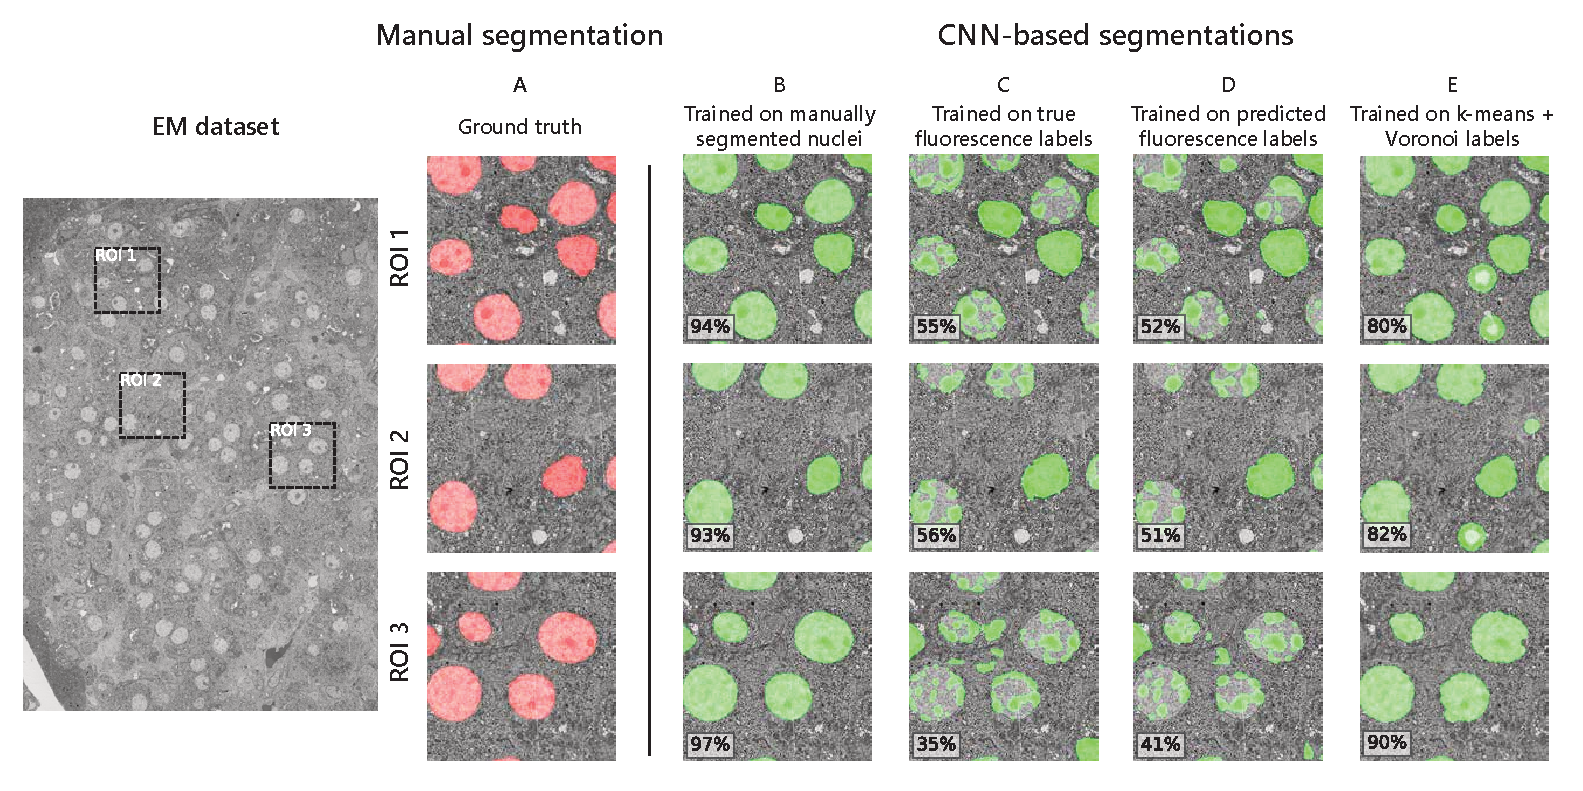
\includegraphics[width=\linewidth]{chapter-4/figures/fig5_segmentation_v3.pdf}
    \caption{\textbf{Semi-automated labelling strategy outperforms [simple thresholding approaches].}
    CNN-based segmentation results for various labelling strategies. Three randomly selected regions of interest are selected from a large-scale EM dataset of rat pancreas tissue to assess segmentation performance. The EM dataset was not included in the training or validation datasets as it was reserved for testing. Intersection-over-union (IoU) scores are provided in the corner of each ROI. CNN architecture for all segmentation results is based on ResNet-34.
    A) Manually segmented cell nuclei serve as ground truth. B) Segmentation results from the traditional approach of training a CNN on nuclei that have been manually segmented yields the best performance at the expense of requiring hours of human annotation time.
    C) Segmentation results from training a CNN on labels automatically generated from correlative fluorescence images reflect the [patchy nature of Hoechst distribution]. Nuclei are segmented with high-precision (very few false positives), but portions of many nuclei are missed (high false negatives).
    D) Training a CNN on labels automatically generated from the predicted fluorescence images results in comparable segmentation performance.
    E) Segmentation results from training a CNN on semi-automatically generated labels based on partial points annotation together with k-means clustering and Voronoi partitioning [results] in improved segmentation performance.
    \textbf{[TODO: Add scale bars.]}}
    \label{fig:4.6_segmentation}
\end{figure}



\clearpage

% Figure 4.S1 (ROIS)
% ------------------
\begin{figure}[!tbh]
    \centering
    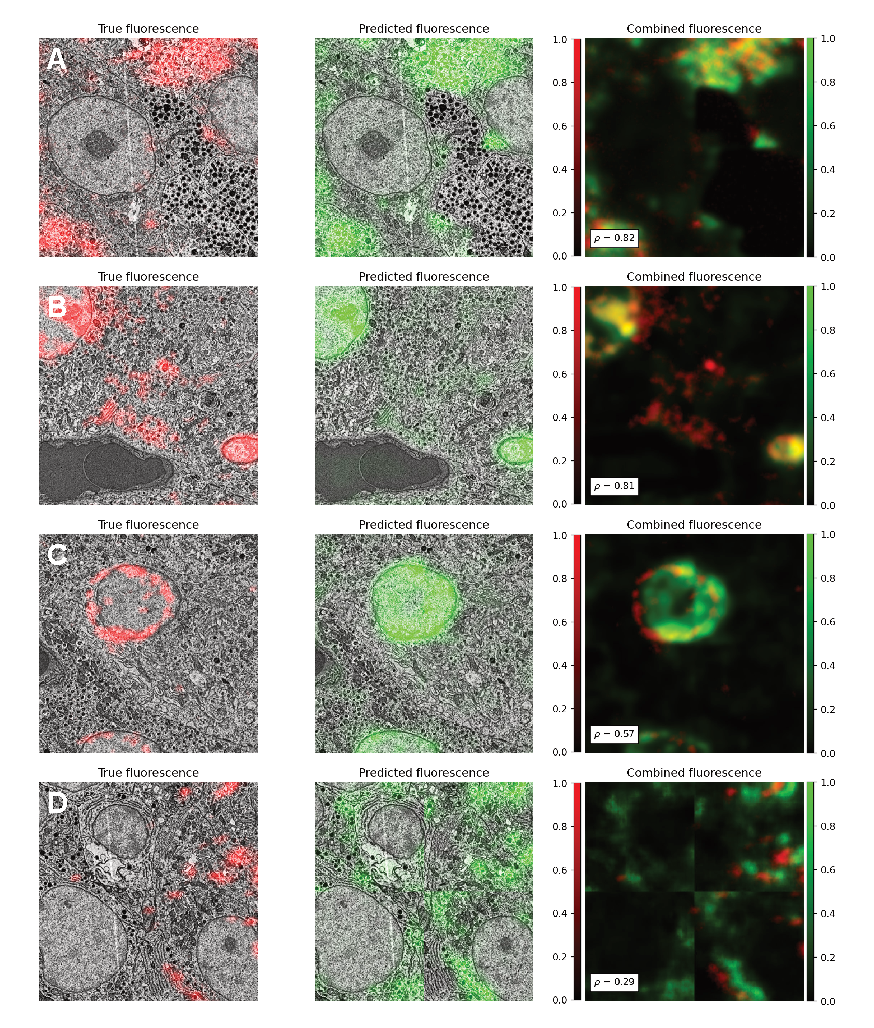
\includegraphics[width=\linewidth]{chapter-4/figures/figS1_rois_v2.pdf}
    \caption{\textbf{The deep CNN developed for fluorescence predictions is able to make distinctions that are nontrivial by eye as well as mitigate issues inherent to fluorescence imaging.}
    For each selected ROI (A-D), the true fluorescence (red) and predicted fluorescence (green) are overlaid onto the EM (columns one and two), and combined to show overlap and differences in signal intensity (column three).
    A) The network is able to distinguish between insulin and similar-looking glucagon granules, a difficult task for non-experts.
    B) An instance of AF594 emission from \SI{405}{\nano\meter} Hoechst excitation demonstrates that the network prediction is not susceptible to such bleedthrough artefacts.
    C) The EM-FM registration occasionally diverges at the corners of the fluorescence field of view due to off-axis, optical aberrations. As the predicted fluorescence is generated directly on structures within the EM image, registration accuracy is determined by the EM pixel size and consistent throughout the dataset. 
    D) Additional off-axis aberrations such as vignetting occasionally result in diminished signal at the corners of the fluorescence field of view. The network is again unaffected by such aberrations for the same reason as in (C).
    \textbf{[TODO: Add scale bars. Transparent PCC box.]}}
    \label{fig:4.S1_rois}
\end{figure}
